\chapter{Аналитический раздел}

В аналитическом разделе подробно рассмотрена предметная область и проанализированы существующие методы. Описана формальная постановка задачи. А так же сформулированы функциональные требования к решению.

%
\section{Задачи тематического моделирования}

Задачи, для решения которых используется тематическое моделирование разбивают на 2 класса: \textbf{Автоматический анализ текста} и \textbf{систематизация больших объемов информации}.

~\

В задачах автоматического анализа текста обычно выделяют следующие направления.

\begin{itemize}
    \item \textbf{Классификация документов} - необходимо присвоить каждому документу метку соответствующих классов.
    \item \textbf{Автоматическое аннотирование документов} - составление краткого обзора документа на основании использования наиболее важных фраз, используя наиболее важные фразы.
    \item \textbf{Автоматическое реферирование или суммаризация коллекции} - решение предыдущей задачи для большой коллекции документов.
    \item \textbf{Тематическая сегментация документов} - разбиение длинного документа на части с различными темами.
\end{itemize}

~\

В задачах систематизации больших объемов информации обычно выделяют следующие направления:

\begin{itemize}
    \item \textbf{Семантический (разведочный) поиск информации} - поиск по коллекции документов на базе тематического моделирования позволяет использовать длинный документ в качестве поискового запроса, а также находить документы, близкие по смыслу, даже если ключевые слова, используемые при поиске, отсутствуют в результатах поиска.
    \item \textbf{Визуализация тематической структуры коллекции} - все задачи, связанные с графическим представлением больших массивов документов.
    \item \textbf{Анализ динамики развития тем} - обычно используется при наличии данных о времени создания документов в коллекции.
    \item \textbf{Тематический мониторинг новых поступлений} - автоматический мониторинг настроенных ресурсов на наличие новых документов, схожих по тематике с настроенным целевым документом.
    \item \textbf{Рекомендация документов пользователям} - создание рекомендательных систем на основании данных о просмотренных пользователем документах и его активности.
\end{itemize}

\begin{figure}[h]
    \center{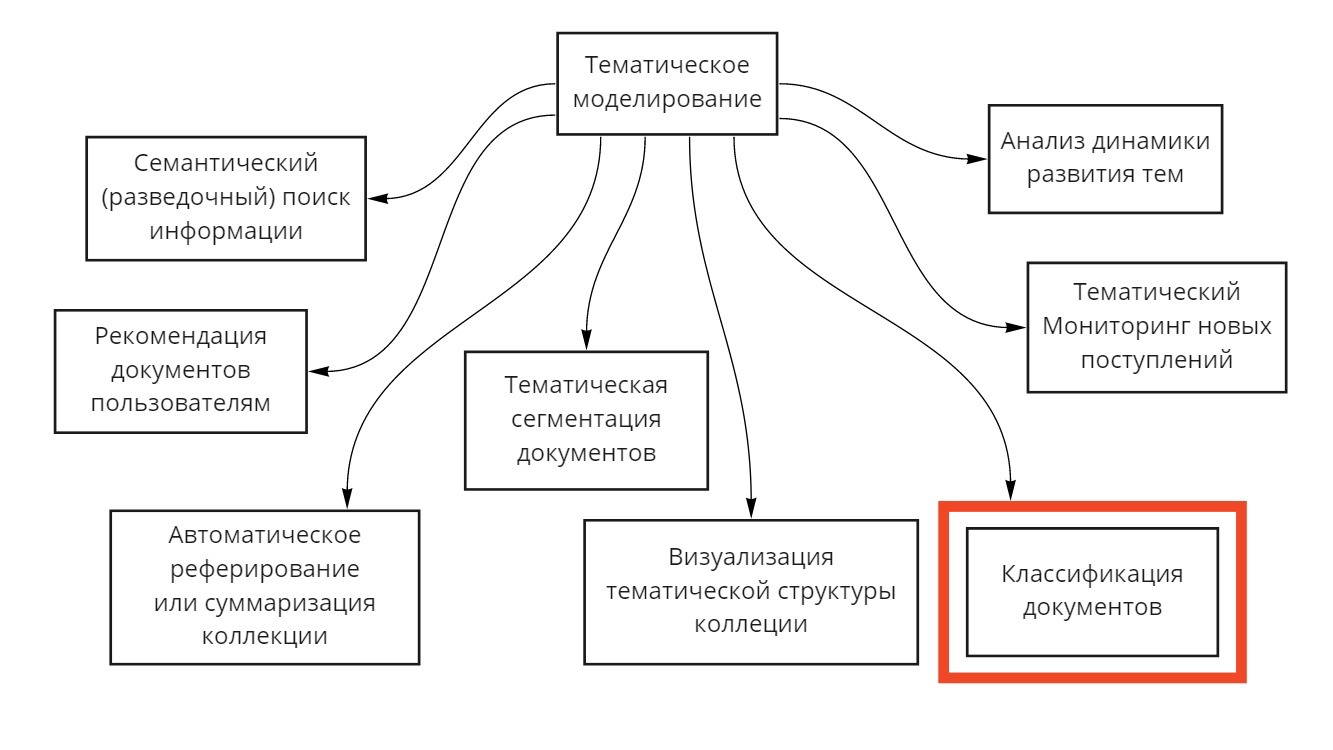
\includegraphics[scale=0.35]{TaskTM.jpeg}}
    \caption{Задачи тематического моделирования.}
    \label{fig:TaskTM}
\end{figure}

%
\section{Существующие методы}

%%
\subsection{Основы кластеризации и классификации документов}

Документы представляются векторной моделью (VSM, Vector Space Model). В такой модели каждому слову сопоставляется определенный вес, вычисляемый по весовой функции.

Базовый вариант весовых функций в таком представлении данных - частота слова (TF), которая равна отношению числа вхождения определенного слова к общему числу слов документа
\begin{equation}
TF(t,d)={{freq(t,d)}\over{max_{W \in D} freq(w,d)}}.
\end{equation}
где

freq() - частота (frequency).

Так же используется агрегирующий показатель
\begin{equation}
TF-IDF(t,d,D)=TF(t,d) \times IDF(t,D),
\end{equation}
где

IDF — обратная частота документа, инверсия частоты, с которой определенное слово встречается в документах коллекции.
\begin{equation}
IDF(t,D)=\log{{|D|}\over{|\{ d \in D:t \in d \}|}}
\end{equation}
где

$|D|$ — число документов в коллекции.

$|\{ d \in D:t \in d \}|$ — число документов из коллекции  $D$, в которых встречается  $t$ (когда $n_t \neq 0$).

Выбор основания логарифма в формуле не имеет значения, поскольку изменение основания приводит к изменению веса каждого слова на постоянный множитель, что не влияет на соотношение весов.


В первый раз задача определения и отслеживания тем (TDT, Topic Detection and Tracking) встречается в работе 
"Topic Detection and Tracking Pilot Study. Final Report" \cite{JamesAllan}. Темой в этой работе называют событие или действие вместе со всеми непосредственно связанными событиями или действиями. Задачей является извлечение событий.

Еще вариант из работы \cite{JamesAllan}:
\begin{equation}
w(t,D)=(1+\log_2{TF(t,D)}) \times {{IDF(t)}\over{||\vec{d}||},}
\end{equation}
где $||\vec{d}||$ - номер вектора, представляющего документ $D$.
\noindentЕще варианты модификаций TF-IDF из работ \cite{Allan}:
\begin{equation}
TF'={{TF}\over{TF+0.5+1.5{{l_d}\over{l_{avg}}}}},
\end{equation}
где $l_d$ - длинна документа $d$, а $l_{avg}$ - средняя длинна документа.
\begin{equation}
IDF'={{\log{(IDF)}}\over{\log{(N+1)}}}
\end{equation}

Для определения расстояния в таком представлении данных использовались различные метрики: дивергенция Кульбака-Лейблера, косинусная мера и другие. В первых работах для решения таких задач использовались алгоритмы кластеризации - выделение групп близких объектов без обучающей выборке и без сведений о классах: метод К-средних, инкрементальная кластеризация, на основе анализа плотности точек \cite{Klyshinskiy1} и т. д.  Каждый кластер описывал то или иное событие.

Главным недостатком такого подхода является однозначность отношения документ-тема. То есть один документ относится к одной теме (событию). В рассматриваемом ниже примере про новость финансирования спорта будет продемонстрировано, что в одном документе могут затрагиваться сразу две темы и футбол и финансы. При таком подходе эти данные теряются.

Используется векторное представление текста, как было сказано выше. Координатой документа может быть частота термина или иных конструкций, полученных при анализе текста. Текст подлежит четырем ключевым этапам анализа - морфологическому, синтаксическому, семантическому \cite{Klyshinskiy2}, графематическому. В качество координат документа в данной работе будем рассматривать частоты употребления в нем слов, представленных леммами - начальными формами слова.

Семантика это раздел лингвистики, изучающий смысловое значение единиц языка.

%%
\subsection{Латентный семантический анализ (LSA)}

Dumais и другие \cite{Dumais1} в 1988 году предложили метод LSA. Суть метода в том, чтобы спроецировать документы и термины в пространство более низкой размерности. Для этого анализируется совместная встречаемость слов (терминов) в документах. Таким образом задача состоит в том, чтобы часто встречающиеся вместе термины были спроецированы в одно и то же измерение семантического пространства.

Этот метод использует мешок слов (или Bag of Words). Это модель текстов на натуральном языке, в которой каждый документ или текст выглядит как неупорядоченный набор слов без сведений о связях между ними. Его можно представить в виде матрицы, каждая строка в которой соответствует отдельному документу или тексту, а каждый столбец — определенному слову.

%%
\subsection{Вероятностный латентный семантический анализ (PLSA)}

В 1999 году Томасом Хофманом был предложен метод вероятностного латентного семантического анализа (PLSA) \cite{Hofmann} \cite{Hofmann1}. В вероятностных тематических моделях, в отличие от рассмотренных выше методов, сначала задается модель, а после с помощью матрицы слов в документах оцениваются ее скрытые параметры. В связи с этим появляется возможность дообучения моделей и упрощается подбор параметров.

Для лучшего понимания алгоритма рассмотрим детальнее процесс написания новости журналистом. Для начала работы он выбирает тему своей новостной статьи. Это, в свою очередь, влияет на то, какие слова он будет использовать. Очевидно, что если журналист решил написать новость про футбол, то слово <<мяч>> в таком документе появится с большей вероятностью, чем слово <<антиматерия>>. При этом если статья затрагивает финансовую сторону вопроса, то вероятности возникновения слов <<мяч>> и слово <<бюджет>> могут сравняться. В таком случае мы можем сказать,  что такая новость имеет минимум две темы - <<спорт>> и <<финансы>>, которые в свою очередь и породили слова <<мяч>> и <<бюджет>>. 

Продолжая эту аналогию, можно представить любую новость как смесь различных тем, которые в свою очередь породили слова. 

\begin{figure}[h]
\center{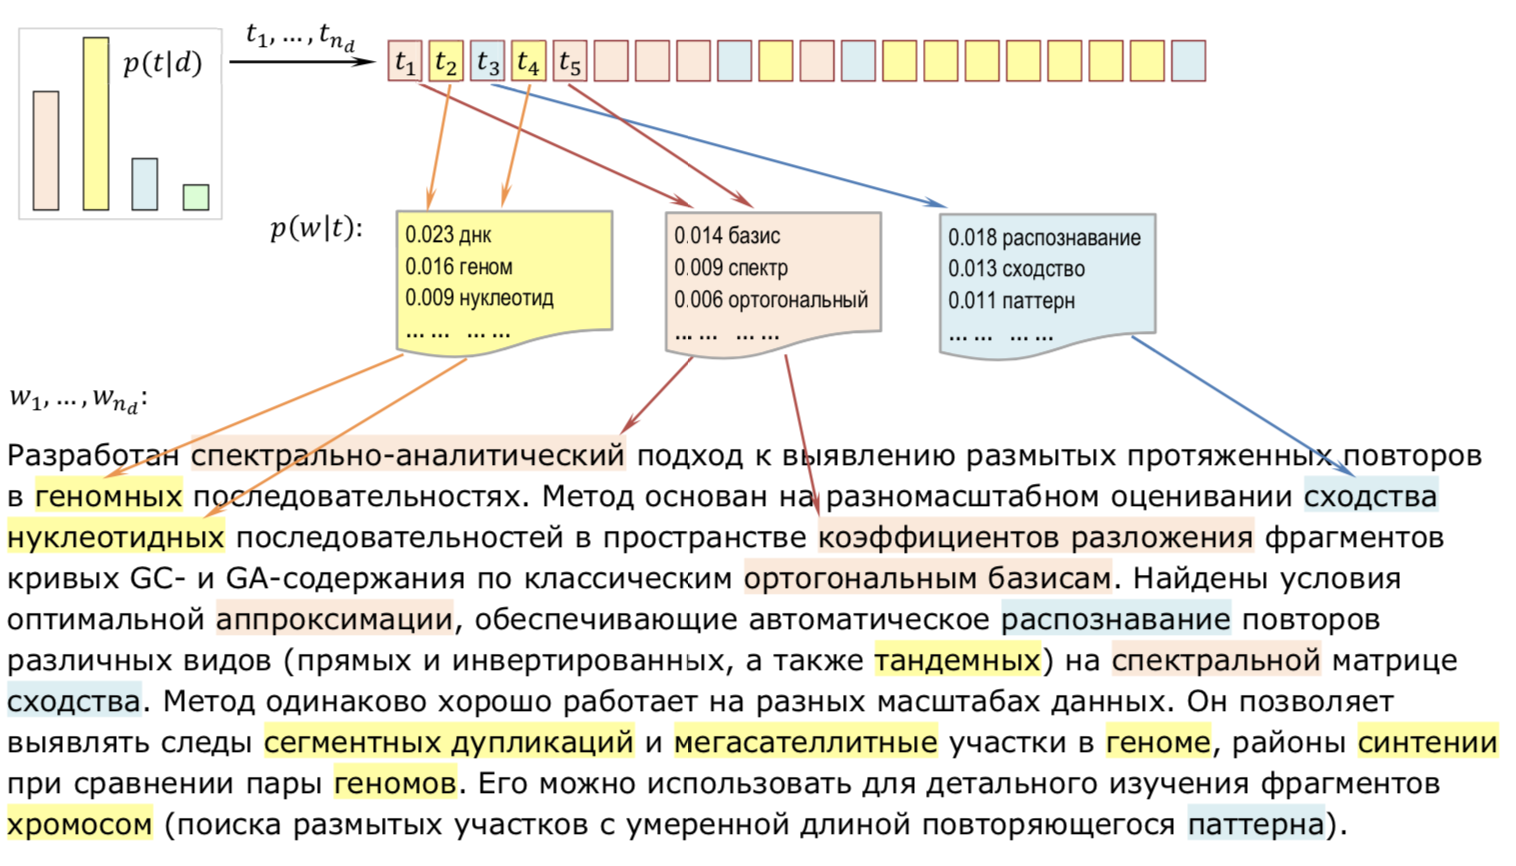
\includegraphics[scale=0.5]{create_text.png}}
\caption{Процесс порождения текстового документа вероятностной тематической моделью. Иллюстрация из лекции К.В. Воронцова}
\label{fig:image}
\end{figure}


\noindentПриняты следующие допущения.

\begin{itemize}
    \item Порядок слов в документе не важен (bag of words).
    \item Слова в документах генерируются темой, а не самим документом.
    \item Порядок документов в коллекции не важен.
    \item Каждое отношение документ-слово $(d,w)$ связано с некоторой темой $t \in T$.
    \item Коллекция представляет собой последовательность троек документ-слово-тема $(d,w,t)$.
    \item В теме невелико число образующих слов.
    \item В документе используется небольшое число тем.
\end{itemize}

~\

\noindentПусть


 $D$ - коллекция документов размера $n_d$ с документами $d$,

 $W$ - словарь терминов размера $n_w$ со словами $w$,

 $T$ - список тем размера размера $n_t$ с темами $t$,

 $n_{dw}$ - количество использований слова $w$ в документе $d$,

 каждый документ состоит из слов: $d \subset W$,

 $p(w|d)$ - вероятность появления слова $w$ в документе $d$,

 $p(w|t)$ - вероятность появления слова $w$ в теме $t$,

 $p(t|d)$ - вероятность появления темы $t$ в документе $d$,

 $\hat{p}(w|d) = {{n_dw}\over{n_d}}$ - наблюдаемая частота слова $w$ в документе $d$.

~\

\noindentТребуется найти параметры вероятностной порождающей тематической модели, то есть представить вероятность появления слов в документе $p(w|d)$ в виде:
\begin{equation}
p(w|d) = \sum_{t \in T}{ p(w|t) p(t|d) }.
\end{equation}
\noindentЗапишем вероятности $p(w|t)$ в матрицу $\Phi=(\phi_{wt})$, а вероятности $p(t|d)$ - в матрицу $\Theta=(\theta_{td})$. Тогда вероятность появления слов в документе можно представить в виде матричного разложения:
\begin{equation}
p(w|d) = \sum_{t \in T}{ \phi_{wt} \theta_{td} }.
\end{equation}

\begin{figure}[h]
\center{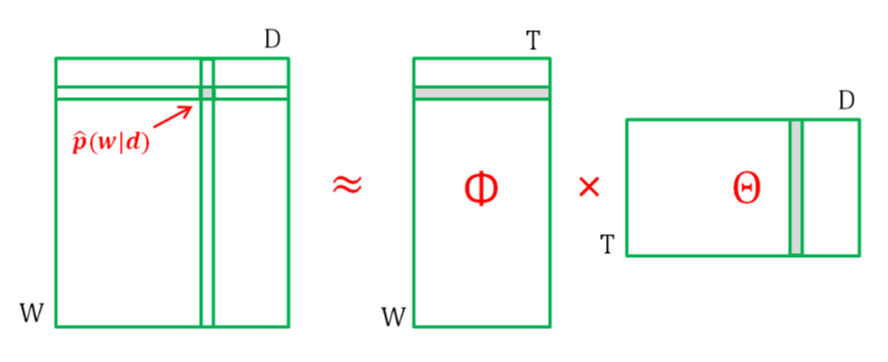
\includegraphics[scale=0.8]{mx.png}}
\caption{Матричное разложение. Иллюстрация из лекции К.В. Воронцова .}
\label{fig:image}
\end{figure}


То есть решается задача, обратная к генерации текста (работе журналиста). Необходимо по имеющийся коллекции документов понять, какими распределениями матриц $\phi_{wt}$ и $\theta_{td}$ она могла быть получена.

Пhи этом так как речь идет о вероятностных тематических моделях каждый столбец матриц $\phi_{wt}$ и $\theta_{td}$ представляет собой дискретное распределение вероятностей. То есть значения не отрицательны и сумма по каждому столбцу равна 1. Такие матрицы называют стохастическими.

Теперь, воспользовавшись принципом максимума правдоподобия с ограничениями на элементы стохастических матриц, если максимизировать  логарифм правдоподобия,получается:

\begin{equation}
\begin{cases}
    \sum_{d \in D} \sum_{w \in d} n_{dw} \ln{\sum_{t \in T} \phi_{wt} \theta_{td} } \rightarrow max_{\Phi,\Theta};\\
    \sum_{w \in W}\phi_{wt} = 1; &\phi_{wt} \ge 0;\\
    \sum_{t \in T}\theta_{td} = 1; &\theta_{td} \ge 0.\\
\end{cases}
\end{equation}

%%
\subsection{Латентное размещение Дирихле (LDA)}

\noindentЗадача в таком виде поставлена не корректно так как существует больше одного решения этой системы:
\begin{equation}
\Phi\Theta = (\Phi S)(S^{-1}\Theta)=\Phi'\Theta'.
\end{equation}
\noindentТо есть результаты будут зависеть от стартовых значений параметров модели и при кадом обучении будут различаться. Но так же это означает, что есть возможность модифицировать алгоритм, сужая пространство решений. Введем для этого критерий регуляризации $R(\Phi,\Theta)$ - некоторый функционал, соответствующий прикладной задаче, для которой обучается модель. Рассмотрим задачу максимизации регуляризованного правдоподобия:

\begin{equation}
\begin{cases}
    \sum_{d \in D} \sum_{w \in d} n_{dw} \ln{\sum_{t \in T} \phi_{wt} \theta_{td} } + R(\Phi,\Theta) \rightarrow max_{\Phi,\Theta};\\
    \sum_{w \in W}\phi_{wt} = 1; &\phi_{wt} \ge 0;\\
    \sum_{t \in T}\theta_{td} = 1; &\theta_{td} \ge 0.\\
\end{cases}
\end{equation}

В 2003 году Дэвидом Блеем, Эндрю Энджи и Маклом Джорданом был предложен метод латентного размещения Дирихле (LDA) \cite{Blei}. На данный момент это одна из самых цитируемых статей по тематическому моделированию. Они предложили решать задачу со следующим регуляризатором:
\begin{equation}
\begin{aligned}
R(\Phi,\Theta) = \sum_{t,w}{(\beta_w-1)\ln{\phi_{wt}}} + \sum_{d,t}{(\alpha_t-1)\ln{\theta_{td}}},\\
\beta_w > 0, \\
\alpha_t > 0,
\end{aligned}
\end{equation}
где $\beta_w$ и $\alpha_t$ - параметры регуляризатора.

Для понимания метода введем понятие дивергенции Кульбака-Лейблера для дискретных распределений.\noindentПусть даны два дискретных распределения $P=(p_i)_{i=1}^n$ и $Q=(q_i)_{i=1}^n$, тогда дивергенция Кульбака-Лейблера выражается так
\begin{equation}
KL(P||Q)=\sum_i{p_i \log{{p_i}\over{q_i}}}.
\end{equation}
Дивергенция Кульбака-Лейблера обладает следующими свойствами.

\begin{itemize}
    \item неотрицательность:
        $$
        KL(P||Q)\ge 0;
        $$
        $$
        KL(P||Q)=0 \Leftrightarrow P=Q
        $$
    \item несимитричность:
        $$
        KL(P||Q)\neq KL(Q||P)
        $$
\end{itemize}

~\

Дивергенция Кульбака-Лейблера связана с максимумом правдоподобия:
\begin{equation}
\sum_{i=1}^{n}p_i\ln{p_i \over {q_i(\alpha)}} \rightarrow \underset{\alpha}{min} \Leftrightarrow \sum_{i=1}^{n}p_i\ln{q_i(\alpha)} \rightarrow \underset{\alpha}{max}
\end{equation}

Минимизация дивергенции Кульбака-Лейблера эквивалентна максимизации правдоподобия. Пусть $P$ - эмпирическое распределение. $Q$ - параметрическая модель распределения с параметром $\alpha$. При минимизации дивергенции Кульбака-Лейблера (максимизации правдоподобия) определяется такое значение $\alpha$, при котором $P$ как можно лучше соответствует модели.

Пусть $\beta=(\beta_w)$ - некоторый вектор над словарем $W$ со словами $w$.

При $\beta_w>1$ вероятность $\phi_{wt}$ этого слова по темам будет сглаживаться, приближаясь к $\beta_w^+$ : 
\begin{equation}
KL(\beta^+||\phi_t) \rightarrow min,
\end{equation}
\begin{equation}
\beta_w^+=\underset{w \in W}{norm}(\beta_w-1)
\end{equation}
При $\beta_w<1$ значение $\phi_{wt}$ наоборот будут разреживаться, удаляясь от $\beta_w^-$ к нулю : 
\begin{equation}
KL(\beta^-||\phi_t) \rightarrow max,
\end{equation}
\begin{equation}
\beta_w^-=\underset{w \in W}{norm}(1-\beta_w)
\end{equation}
то есть в матрице $\Phi$ будет больше нулевых элементов или близких к нулю.

%%
\subsection{Аддитивная регуляризация тематических моделей (ARTM)}

Неединственность решения максимизации регуляризованного правдоподобия позволяет накладывать сразу несколько ограничений на модель, этот метод называется аддитивной регуляризацией тематических моделей (ARTM).

То есть
\begin{equation}
\sum_{d,w}{n_{dw} \ln{\sum_t\phi_{wt} \theta_{td}}} + \sum_{i=1}^k \tau_i R_i(\Phi,\Theta) \rightarrow \underset{\Phi\Theta}{max}
\end{equation}
где $\tau_i$ - коэффициенты регуляризации, а $R_i(\Phi,\Theta)$ - регуляризаторы.

При таком подходе возникает проблема поиска коэффициентов, которая обычно решается добавлением регуляризаторов в модель по одному и оптимизации соответствующих коэффициентов в ходе пробных запусков моделей.

%%
\subsection{Решение задачи максимизации регуляризованного правдоподобия}

Решение задачи в общем виде аналитическими методами слишком сложно. Однако, если выбирать гладкие регуляризаторы, то можно воспользоваться условием Крауша-Куна-Таккера. Получится система уравнений:
\begin{equation}
\begin{cases}
    p_{tdw} = \underset{t \in T}{norm}(\phi_{wt} \theta_{td}) \\
    \phi_{wt} = \underset{w \in W}{norm}\bigg( \underset{d \in D}\sum{n_{dw} p_{tdw} + \phi_{wt} {{\partial R} \over {\partial \phi_{wt}}}} \bigg) \\
    \theta_{td} = \underset{t \in T}{norm}\bigg( \underset{w \in d}\sum{n_{dw} p_{tdw} + \theta_{td} {{\partial R} \over {\partial \theta_{td}}}} \bigg) \\
\end{cases}
\end{equation}
где
\begin{equation}
\underset{t \in T}{norm}(x_t) = {{max\{ x_t, 0 \}} \over {\underset{s \in T}\sum{ max\{ x_s, 0 \}} }}
\end{equation}

Такую систему можно решить численным методом простых итераций. В данном случае его называют  ЕМ-алгоритм.

Для получения результата необходимо итерационно выполнять Е-шаг и М-шаг до достижения требуемой точности.

Е-шаг :
\begin{equation}
p_{tdw}=\underset{t \in T}{norm}(\phi_{wt} \theta_{td})
\end{equation}

М-шаг : 
\begin{equation}
\phi_{wt} = \underset{w \in W}{norm}\bigg( \underset{d \in D}\sum{n_{dw} p_{tdw} + \phi_{wt} {{\partial R} \over {\partial \phi_{wt}}}} \bigg)
\end{equation}
\begin{equation}
\theta_{td} = \underset{t \in T}{norm}\bigg( \underset{w \in d}\sum{n_{dw} p_{tdw} + \theta_{td} {{\partial R} \over {\partial \theta_{td}}}} \bigg)
\end{equation}

Этот процесс можно организовать параллельно, если обновлять матрицу   $\Phi$ по порциям, после анализа очередного пакета документов. Обычно уже после просмотра нескольких первых десятков тысяч документов матрица $\Phi$ получается уже устоявшиеся и остается только тематизировать остальные документы. Подробнее с EM алгоритмом можно ознакомится в работе Frei O., Apishev M. \cite{EMonline}.

%%
\subsection{Выбор алгоритма}

В данной работе рассматривается задача классификации документов. В качестве документов выступают новости на русском языке. Необходимо с помощью выбранного метода и способов его усовершенствования разбить коллекцию новостей на темы, интерпретируемые человеком и получить возможность оценивать новый документ (новость) на принадлежность этим темам.

Особенностью тематического моделирования является возможность не использовать в процессе построения модели размеченные данные. То есть темы, на которые разбивается коллекция, также создаются в процессе формирования модели.

Для дальнейшей работы принято решение использовать ARTM в качестве базового алгоритма так как он оставляет исследователю много свободы в выборе регуляризаторов, из комбинации и коэффициентов.

\begin{figure}[h]
    \center{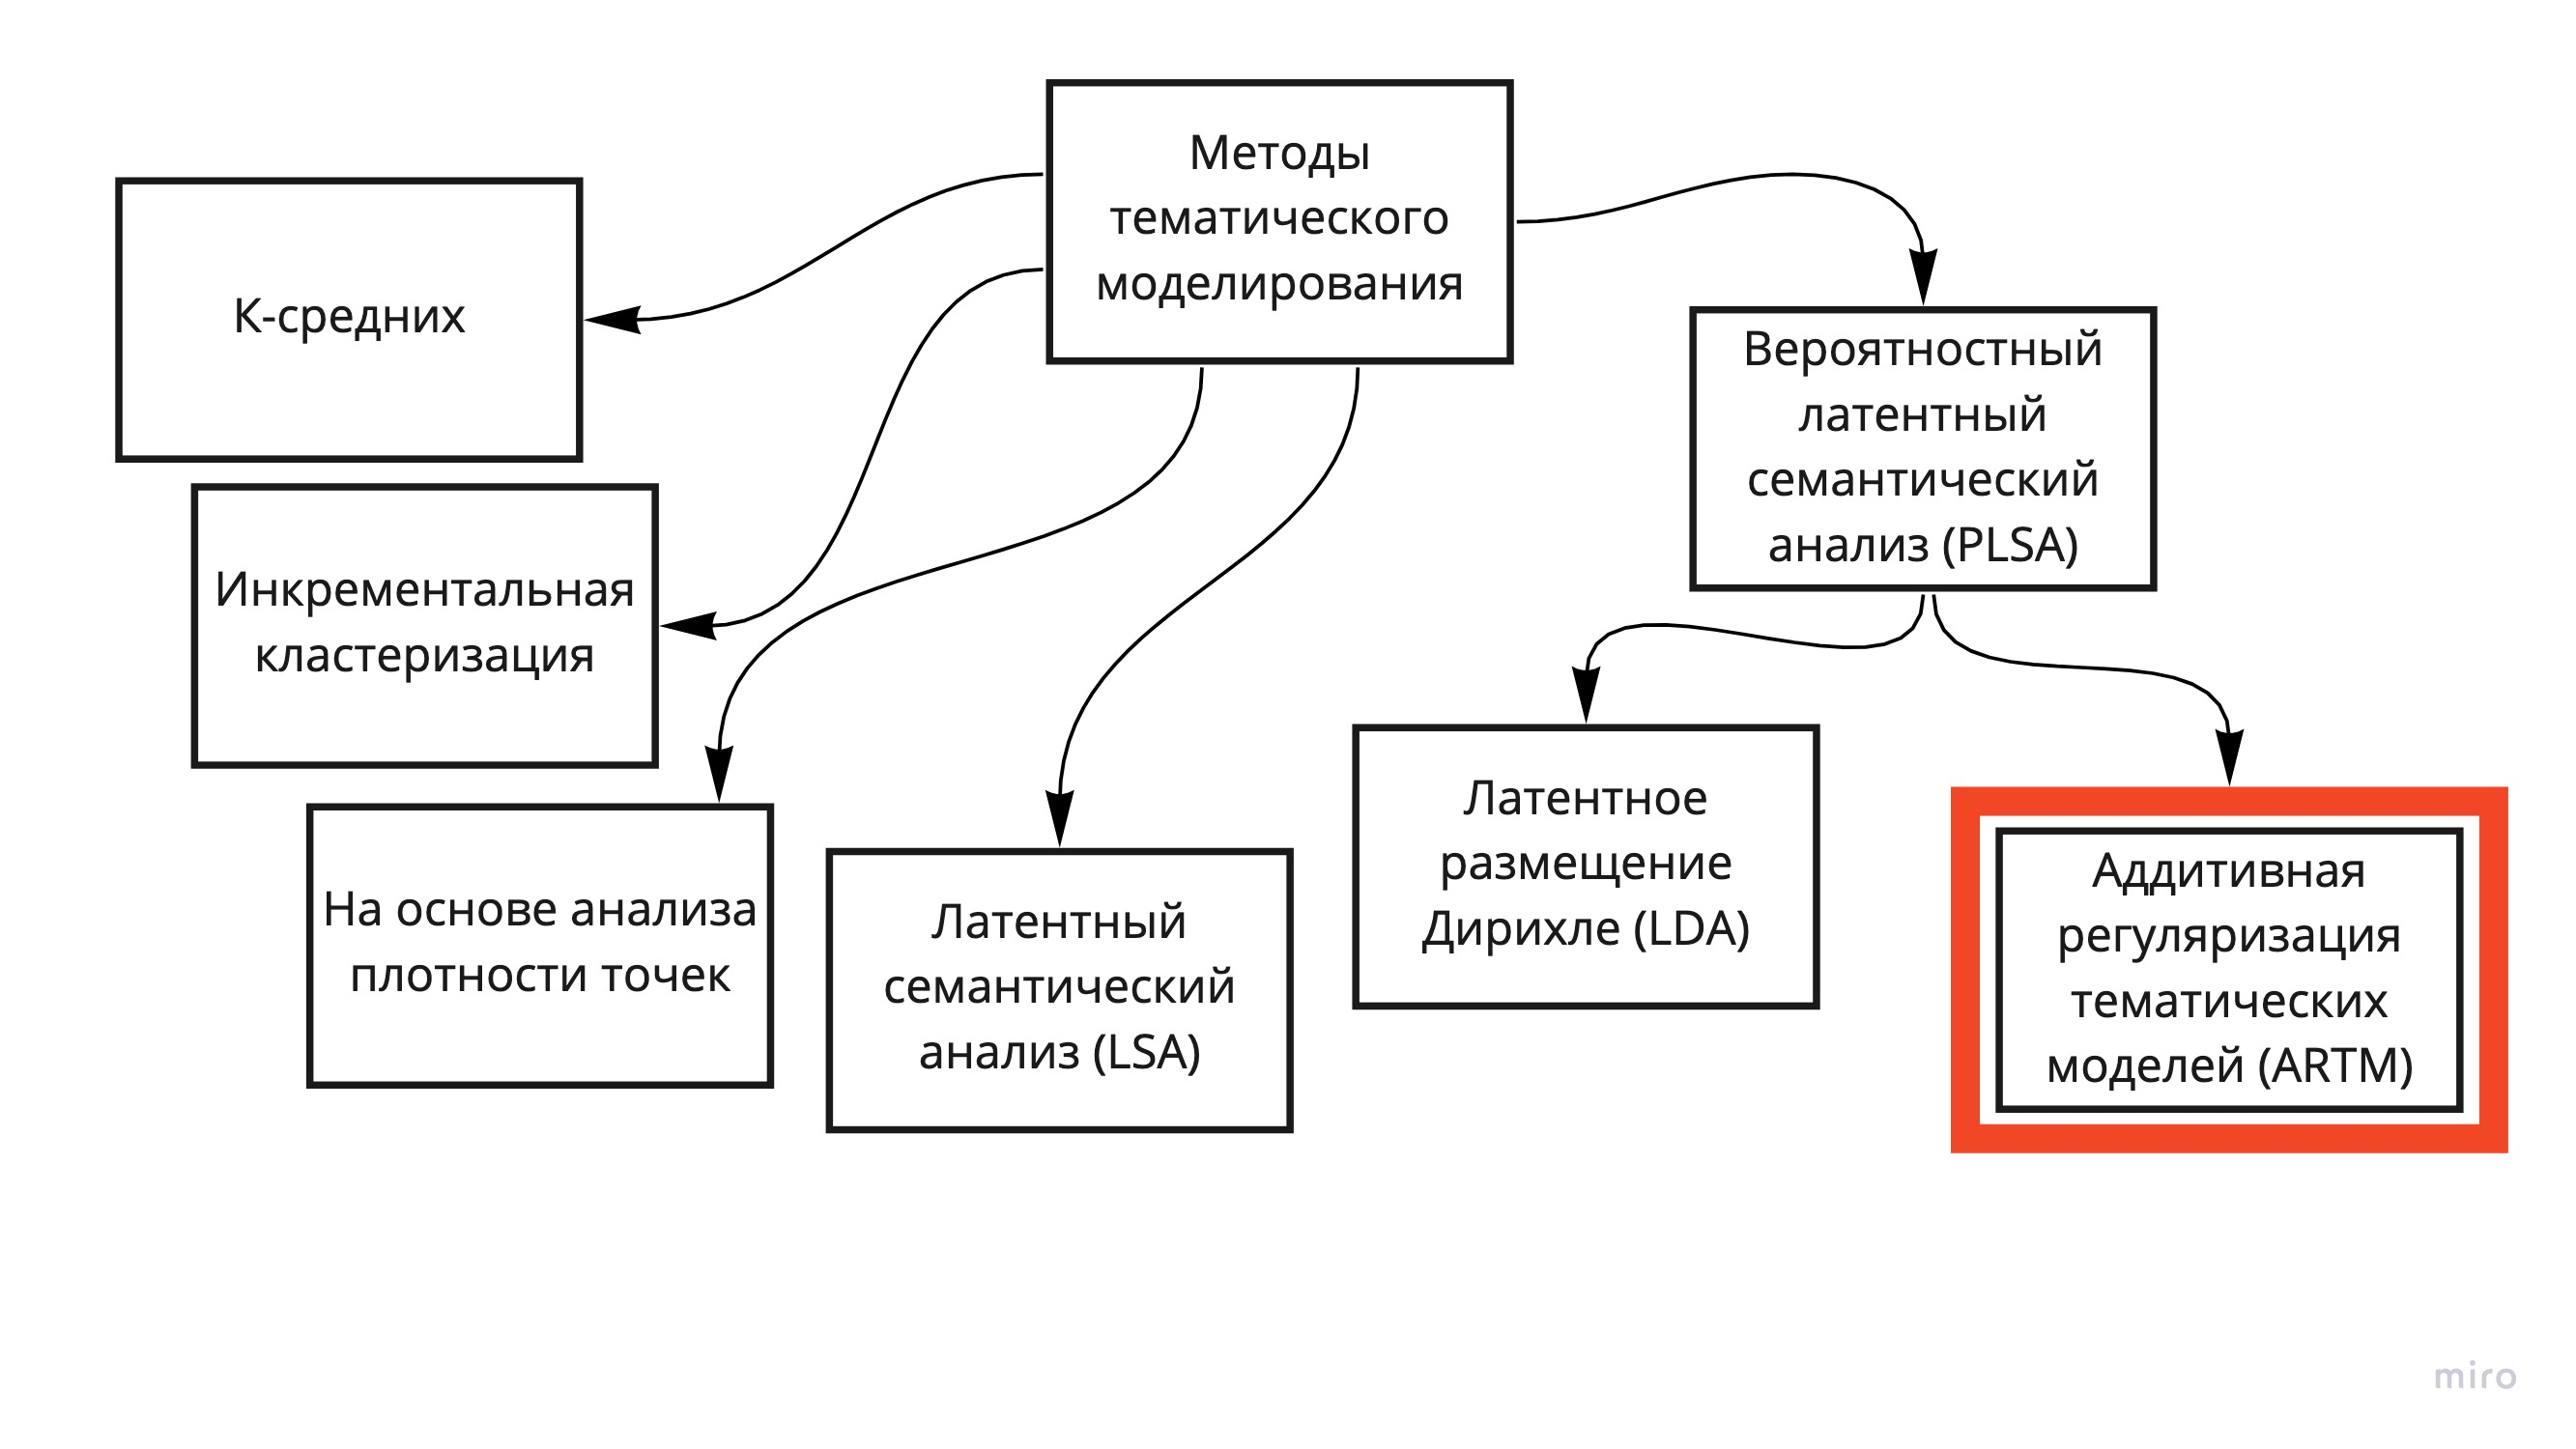
\includegraphics[scale=0.17]{MetodTM.jpeg}}
    \caption{Методы тематического моделирования.}
    \label{fig:MetodTM}
\end{figure}

%%
\section{Формализованное описание проблемы}

\noindentВходные данные:

\begin{itemize}
    \item коллекция новостей на русском языке на разные темы в сети интернет.
\end{itemize}

~\

\noindentВыходные данные:

\begin{itemize}
    \item обученная тематическая модель с настроенными регуляризаторами;
    \item список тем с образующими их словами.
\end{itemize}

~\

\noindentПолучение данных:

\begin{itemize}
    \item парсинг новостных агрегаторов;
    \item парсинг крупных новостных сайтов.
\end{itemize}

~\

\noindentПодготовка данных:

\begin{itemize}
    \item удаление форматирования текста;
    \item исправление опечаток;
    \item слияние слишком коротких текстов;
    \item выделение терминов;
    \item приведение слов к нормальной форме (лемматизация);
    \item удаление слишком частых слов;
    \item удаление слишком редких слов.
\end{itemize}

%
\section{Функциональные требования}

Для решения задачи классификации и категоризации новостей на русском языке необходимо следующее: 

\begin{itemize}
    \item собирать новости из ресурсов сети Интернет;
    \item преобразовывать их в необходимый формат;
    \item создавать и обучать модель;
    \item провести параметризацию: подобрать наилучший комплект регуляризаторов, их параметров и коэффициентов;
    \item иметь возможность последующего повторного использования и дообучения модели.
\end{itemize}
